\subsection{Критическая интенсивность}

    Критической интенсивностью называется такое значение интенсивности, при котором стохастическая траектория выходит за границы бассейна притяжения детерминированного аттрактора и за конечное число итераций стабилизируется в равновесии \(x = 0\).

    Критическая интенсивность может быть получена эмпирически на большом количестве экспериментов. Однако это времезатратный подход. Для теоретической оценки критической интенсивности используется полоса рассеивания построенная с использованием функции стохастической чувствительности. Идея состоит в нахождении такого значения интенсивности шума, при котором доверительный интервал выходит за границы бассейна притяжения аттрактора для модели (\ref{origin}), как было показано в разделе про бифуркационную диаграмму для детерминированного случая на рисунке \ref{bifurcation_attractor} бассейн притяжения аттрактора ограничивается снизу неустоцчивым равновесием \(x_1^*\) и сверху \(x_{-1}^*\), пожтому доверительная полоса будет пересекать бассейн по одной из этих двух границ.

    На рисунке \ref{critical_intensity_beta_noise} изображен график критической интенсивности для \(\beta\)-шума. Красным показана критическая интенсивность для границ доверительных интервалов, которые лежат ниже устойчивого равновесия. Синим - для границ, которые выше устойчивого равновесия. 

    \comment{Для 4-цикла сделать шаг меньше и подойти ближе к 2-циклу. Холмик должен получится}

    \begin{figure}
        \centering
        \subfloat[Модель (\ref{alpha_chaos}) (с \(\alpha\)-шумом)]{
            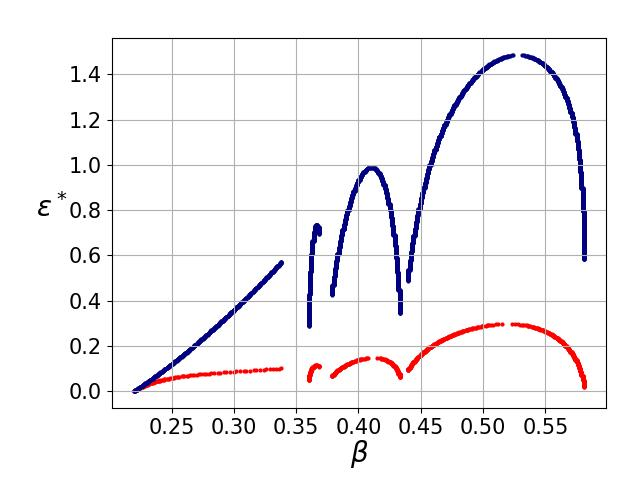
\includegraphics[width=0.55\textwidth]{stochastic/images/critical_intensity_alpha_noise.jpg}
            \label{critical_intensity_alpha_noise}
        }
        \subfloat[Модель (\ref{beta_chaos}) (с \(\beta\)-шумом)]{
            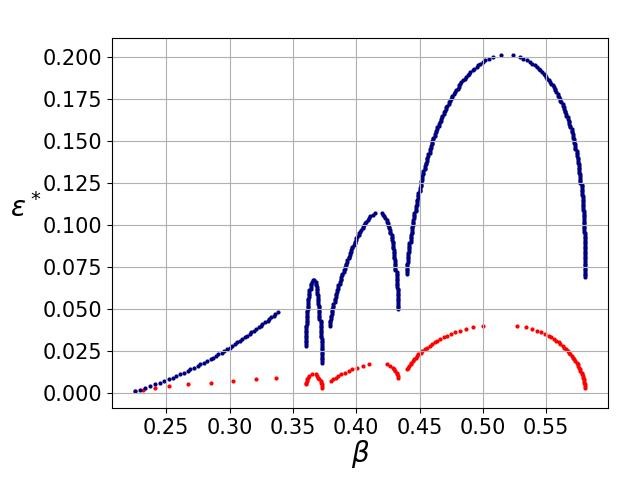
\includegraphics[width=0.55\textwidth]{stochastic/images/critical_intensity_beta_noise.jpg}
            \label{critical_intensity_beta_noise}
        }
        
        \subfloat[Модель (\ref{additive_chaos}) (с аддитивным шумом)]{
            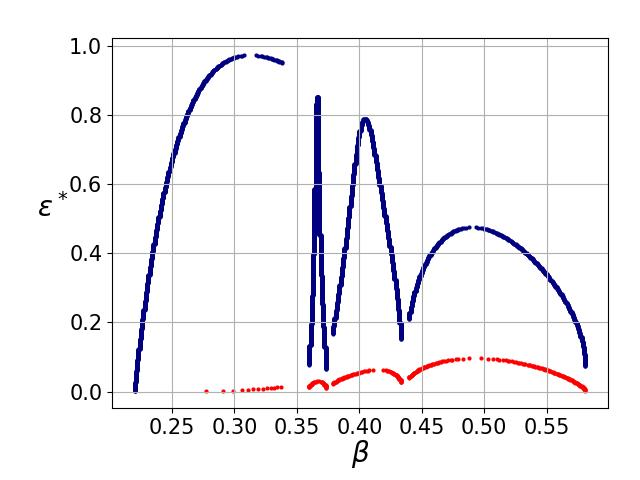
\includegraphics[width=0.55\textwidth]{stochastic/images/critical_intensity_additive_noise.jpg}
            \label{critical_intensity_additive_noise}
        }
            
        \caption{Критическая интенсивность}
    \end{figure}
    
    Обозначения аналогичны для графиков \(\alpha\)-шума (\ref{critical_intensity_alpha_noise}) и аддитивного шума (\ref{critical_intensity_additive_noise}).

    Интересно заметить, что в случае \(\alpha\)-шума и \(\beta\)-шума силуэты графиков очень похожи. В то же время график для аддитивного шума не похож на предыдущие случаи. В этом случае для хаотического аттрактора требуется большая интенсивность, чем для циклов и равновесия. \comment{Как оно связно с ФСЧ?}
